\documentclass[xcolor={dvipsnames,rgb}, aspectratio=169]{beamer}

%%% PACKAGES %%%
\usepackage[T1]{fontenc}
\usepackage{tgheros}

% Metropolis customization
\usetheme[sectionpage=none]{metropolis}
\setbeamercolor{background canvas}{bg=white}
\setbeamercolor{frametitle}{bg = white, fg=black}
\setbeamertemplate{sections/subsections in toc}[square]
\setbeamertemplate{footline}{
   \textcolor{bluepoli}{\rule{\paperwidth}{1pt}}
   \vskip4pt
   \hskip5pt \tiny Root finding (Pt. 1) $|$ Calcoli di Processo dell' Ingegneria
   Chimica \hskip260pt \insertframenumber
   \vskip4pt
}

% color
\usepackage{color}
\usepackage{xcolor}
\usepackage{colortbl}
\definecolor{bluepoli}{cmyk}{0.4,0.1,0,0.4}
\definecolor{mygreen}{RGB}{1, 121,111}
\definecolor{myred}{RGB}{220, 20, 60}
\definecolor{mygreen}{RGB}{28,172,0}
\definecolor{mylilas}{RGB}{170,55,241}
\definecolor{codegreen}{rgb}{0,0.6,0}
\definecolor{codegray}{rgb}{0.5,0.5,0.5}
\definecolor{codepurple}{rgb}{0.58,0,0.82}
\definecolor{backcolour}{rgb}{0.95,0.95,0.92}
\definecolor{lightblue}{rgb}{56, 167, 232}

\colorlet{colorp}{NavyBlue}
\colorlet{colorT}{WildStrawberry}
\colorlet{colork}{OliveGreen}
\colorlet{colorM}{RoyalPurple}
\colorlet{colorNb}{Plum}
\colorlet{colorIs}{black}
\newcommand{\highlight}[2]{\colorbox{#1!17}{$#2$}}
\newcommand{\highlightdark}[2]{\colorbox{#1!47}{$#2$}}

% tikz
\usepackage{tikz}
\usetikzlibrary{positioning}
\usetikzlibrary{backgrounds}
\usetikzlibrary{arrows,shapes}
\usetikzlibrary{tikzmark}
\usetikzlibrary{calc}

% tcolorbox env
% Coloured box for styling theorems, proof, definitions
\usepackage[most]{tcolorbox}

\newtcolorbox{code}[2][]{
    enhanced jigsaw,
    colframe=bluepoli,
    interior hidden, 
    breakable,
    before skip=10pt,
    after skip=10pt
}

% URL and Hyperref
\usepackage{hyperref}
\hypersetup{
    colorlinks=true,
    linkcolor=blue,
    filecolor=magenta,
    urlcolor=blue,
    pdftitle={Overleaf Example},
    pdfpagemode=FullScreen,
}
\usepackage{url}

% Math stuff
\usepackage{amsmath}
\usepackage{amssymb}
\usepackage{mathtools}
\usepackage{blkarray}
\usepackage{multirow}

% Wrapfig
\usepackage{wrapfig}

% Bibliography
\usepackage[
backend=biber,
style=alphabetic,
sorting=ynt
]{biblatex}
\addbibresource{bibliography.bib}

%%% TITLE %%%
\title{Root Finding.\\Part 1}
\subtitle{Calcoli di Processo dell' Ingegneria Chimica}
\author[Dinelli, Mehl]{\textbf{Timoteo~Dinelli}, \textbf{Marco~Mehl}}
\institute{
   \inst{} Department of Chemistry, Materials and Chemical Enginering, G. Natta.
   Politecnico di Milano.\\
   email: timoteo.dinelli@polimi.it \\
   email: marco.mehl@polimi.it \\
}
\date{7\textsuperscript{th} of November 2024.}

\newcommand{\norm}[1]{\left\lVert#1\right\rVert}

\begin{document}
% external files inclusion
% Double underline
\def\doubleunderline#1{\underline{\underline{#1}}}

% \newcommand{\zm}{%
%    \begin{bmatrix}
%       X_{11} & X_{12} & \cdots & X_{1p} \\
%       X_{12} & X_{22} & \cdots & X_{2p} \\
%       \vdots & \vdots & \tikzmarknode{Is}{\highlight{colorT}{X_{ij}}} & \vdots \\
%       X_{n1} & X_{n2} & \cdots & X_{np} \\
%    \end{bmatrix}%
% }

\makeatletter
\newcommand{\DrawLine}{%
  \begin{tikzpicture}
  \path[use as bounding box] (0,0) -- (\linewidth,0);
  \draw[color=bluepoli,dashed,dash phase=2pt]
        (0-\kvtcb@leftlower-\kvtcb@boxsep,0)--
        (\linewidth+\kvtcb@rightlower+\kvtcb@boxsep,0);
  \end{tikzpicture}%
  }
\makeatother

{%
   \setbeamertemplate{footline}{}
   \begin{frame}{}
      \maketitle
      \begin{tikzpicture}[overlay, remember picture]
         \node[above left=6.5cm and .01cm of current page.south east] {
         \includegraphics[trim=1cm 1cm 1.5cm 1cm, clip=true, width=6cm]{
            ./../../Introduction to Matlab/slides/figures/_static/ING_IND_INF-eps-converted-to.pdf
         }
      };
      \end{tikzpicture}
   \end{frame}
}

\begin{frame}{Root Finding}
   \begin{columns}
      \column{0.5\textwidth}
         We will discuss different general algorithms that seek to find the solution
         $\textbf{x}$ of the following canonical equation:
         \begin{equation*}
            f(\textbf{x}) = 0
         \end{equation*}
      \column{0.5\textwidth}
         \begin{figure}
            \centering
            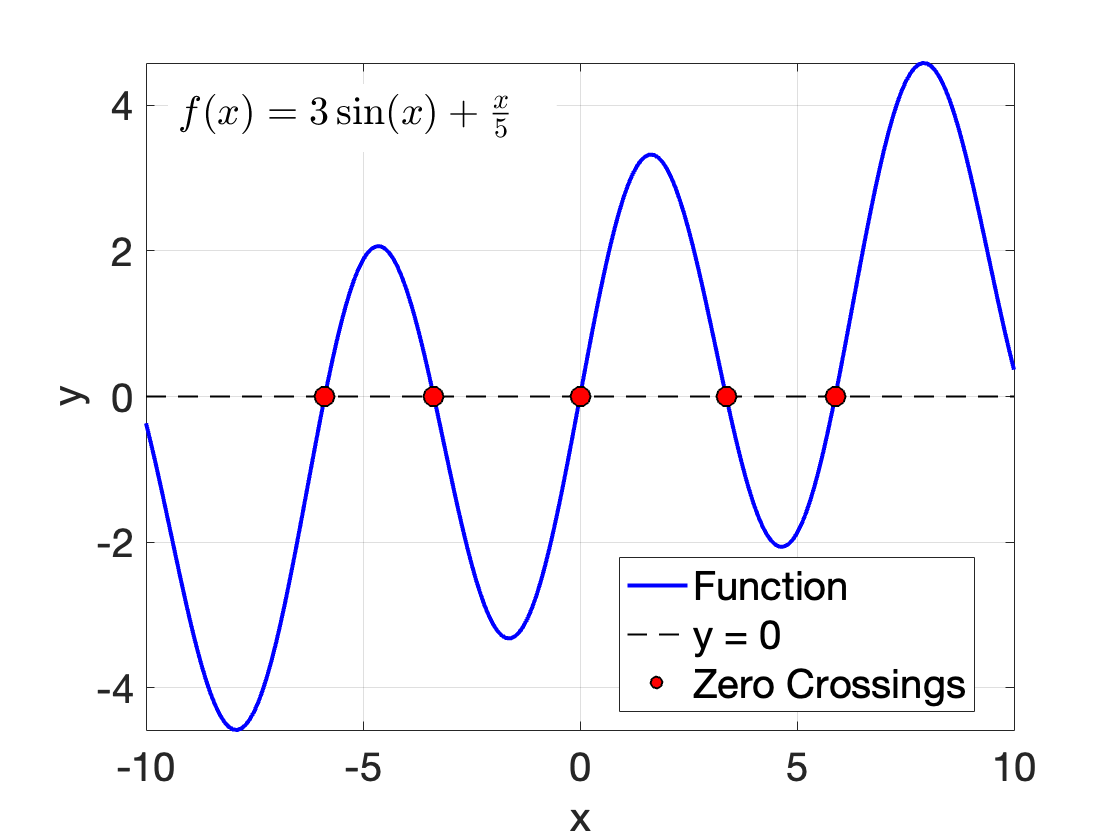
\includegraphics[width=1.\textwidth]{figures/untitled.png}
         \end{figure}
   \end{columns}
\end{frame}

\begin{frame}{General strategy}
   \begin{equation*}
      f(\textbf{x}) = 0
   \end{equation*}
   \begin{enumerate}
      \item Make a (reasonable) first guess ($x_{0}$) or first guesses ($x_0$, $x_1$).
      \item Test the value of $f(x_{0})$.
      \item Then make a new \alert{INTELLIGENT} guess, based on $x_{0}$ and $f(x_{0})$.
      \item Repeat this process, as long as, the required precision on the function value
         is close to selected tolerance $\epsilon_{f}$:
         \begin{equation*}
            \left\lVert f(x_{i+1}) \right\lVert < \epsilon_{f}
         \end{equation*}
         and the solution was found to be convergent.
         \begin{equation*}
            \left\lVert x_{i+1} - x_{i} \right\lVert < \epsilon_{x}
         \end{equation*}
   \end{enumerate}
\end{frame}

\begin{frame}{Bisection method}
   \small{
      Under the hypothesis of Bolzano's theorem, if a function $f(x)$ is continuous in
      the interval $\left[a,\:b\right]$ and takes values of opposite sign at the boundary
      of such interval, then it has a root in that interval.
   }

   Starting with an interval $[a,\: b]$, $f(x)$ and a tolerance $\epsilon$ such that
   $\norm{c - \hat{c}} < \epsilon$. Where $\hat{c}$ is the zero of our function.
   \begin{enumerate}
      \item Compute $c = \frac{a+b}{2}$.
      \item If $b-c \leq \epsilon$ then $c$ is the solution and stop otherwise go to the
         next point.
      \item If $sign\left(f(b)\right) \times sign\left(f(a)\right) \leq 0$ then $a = c$,
         else $b = c$, then go back to point 1 and repeat.
   \end{enumerate}
\end{frame}

\begin{frame}{Newton method}
   \begin{enumerate}
      \item Make a reasonable first guess $x_{0}$.
      \item Compute the next guess according to the following iterative formula:
         \begin{equation*}
            x_{i+1} = x_{i} - \frac{f(x_{i})}{f^{'}(x_{i})}
         \end{equation*}
      \item Repeat the loop till the required precision is reached.
   \end{enumerate}
   \centering
   \alert{Problem}

   How do we compute $f^{'}(x_{i})$?
\end{frame}

\begin{frame}{Newton method}
   \begin{enumerate}
      \item Make a reasonable first guess $x_{0}$.
      \item Compute the next guess according to the following iterative formula:
         \begin{equation*}
            x_{i+1} = x_{i} - \frac{f(x_{i})}{f^{'}(x_{i})}
         \end{equation*}
      \item Repeat the loop till the required precision is reached.
   \end{enumerate}
   \centering
   \alert{Problem}

   How do we compute $f^{'}(x_{i})$?
\end{frame}

\begin{frame}{Derivatives}
   \textbf{Classical} analysis:
      \begin{equation*}
         f^{'}(x_{0}) = \underset{h \longrightarrow 0}{lim}\frac{f(x_{0} + h) - f(x_{0})}{h}
      \end{equation*}

   \textbf{Numerical} analysis: pick a small value for h (e.g. $1*10^{-7})$:
   \begin{equation*}
      f^{'}(x_{0}) = \frac{f(x_{0} + h) - f(x_{0})}{h}
   \end{equation*}
\end{frame}

\begin{frame}{Secant method}
   \vspace{-.5cm}
   \small{
      The newton method tries to simplify the solution of the base problem $f(x) = 0$ using
      the tangent as an approximation of the function we are trying to zero. Assuming to
      know the value of the function $f(x)$ for two distinct values of $x$ ($x_0$ and $x_1$)
      close enough to the solution $\alpha$:
      \begin{enumerate}
         \item Make a reasonable first guess $x_{0}$ and $x_{1}$.
         \item Compute the values $f(x_0)$ and $f(x_1)$ then given the secant equation
            compute the value of $x_2$.
            \begin{equation*}
               x_2 = x_1 - \frac{f(x_1)}{\frac{f(x_1) - f(x_0)}{x_1 - x_0}}
            \end{equation*}
            Then loop until convergence.
      \end{enumerate}
      Generalizing we get the \alert{secant method} based on the following iterative
      formula:
      \begin{equation*}
         x_{n+1} = x_{n} - \frac{f(x_{n})}{\frac{f(x_n) - f(x_{n-1})}{x_n - x_{n-1}}}
      \end{equation*}
   }
\end{frame}

\begin{frame}{Regula falsi method}
   The {\it regula falsi} method is similar to the secant method and to the bisection
   method. This method uses secants and a succession of points as the secant method, but
   throws in in the mix the uncertainty interval represented by two extremes where the
   function to be zeroed (which is assumed to be continuous) has opposite signs. Along the
   iterations, the two points determine the boundaries of the uncertainty interval.
\end{frame}

{%
   \setbeamertemplate{footline}{}
   \begin{frame}[standout]
	   Exercises
   \end{frame}
}

\begin{frame}{Exercise}
   \begin{itemize}
      \item[$\blacktriangleright$] Let's implement the \alert{Bisection} and
         \alert{Newton} method to find the zero of a function. Test them against $f(x) =
         3e^{x} - 4cos(x)$
      \item[$\blacktriangleright$] (Exam 05/02/19, Exercise 4): Find the root of the
         function $f(x) = \frac{1}{x-2} - 2$. After several attempts it can be noticed
         that the Newton method fails for first guesses as $x_{0} = 1.8$ and $x_{0} = 4$,
         while converge rapidly if the first guess is equal to $x_{0} = 2.2$. Explain why
         this happens using also a graphical representation, determine the interval where
         is possible to identify a first guess that allows the method to converge.
         Compute the solution using Newton method and Bisection method with a precision
         of $1e^{-2}$. Then compare the results obtained with the Matlab's built-in
         method \textcolor{blue}{fzero} and \textcolor{blue}{fsolve}.
   \end{itemize}
\end{frame}

\begin{frame}{}
   \begin{figure}
      \centering
      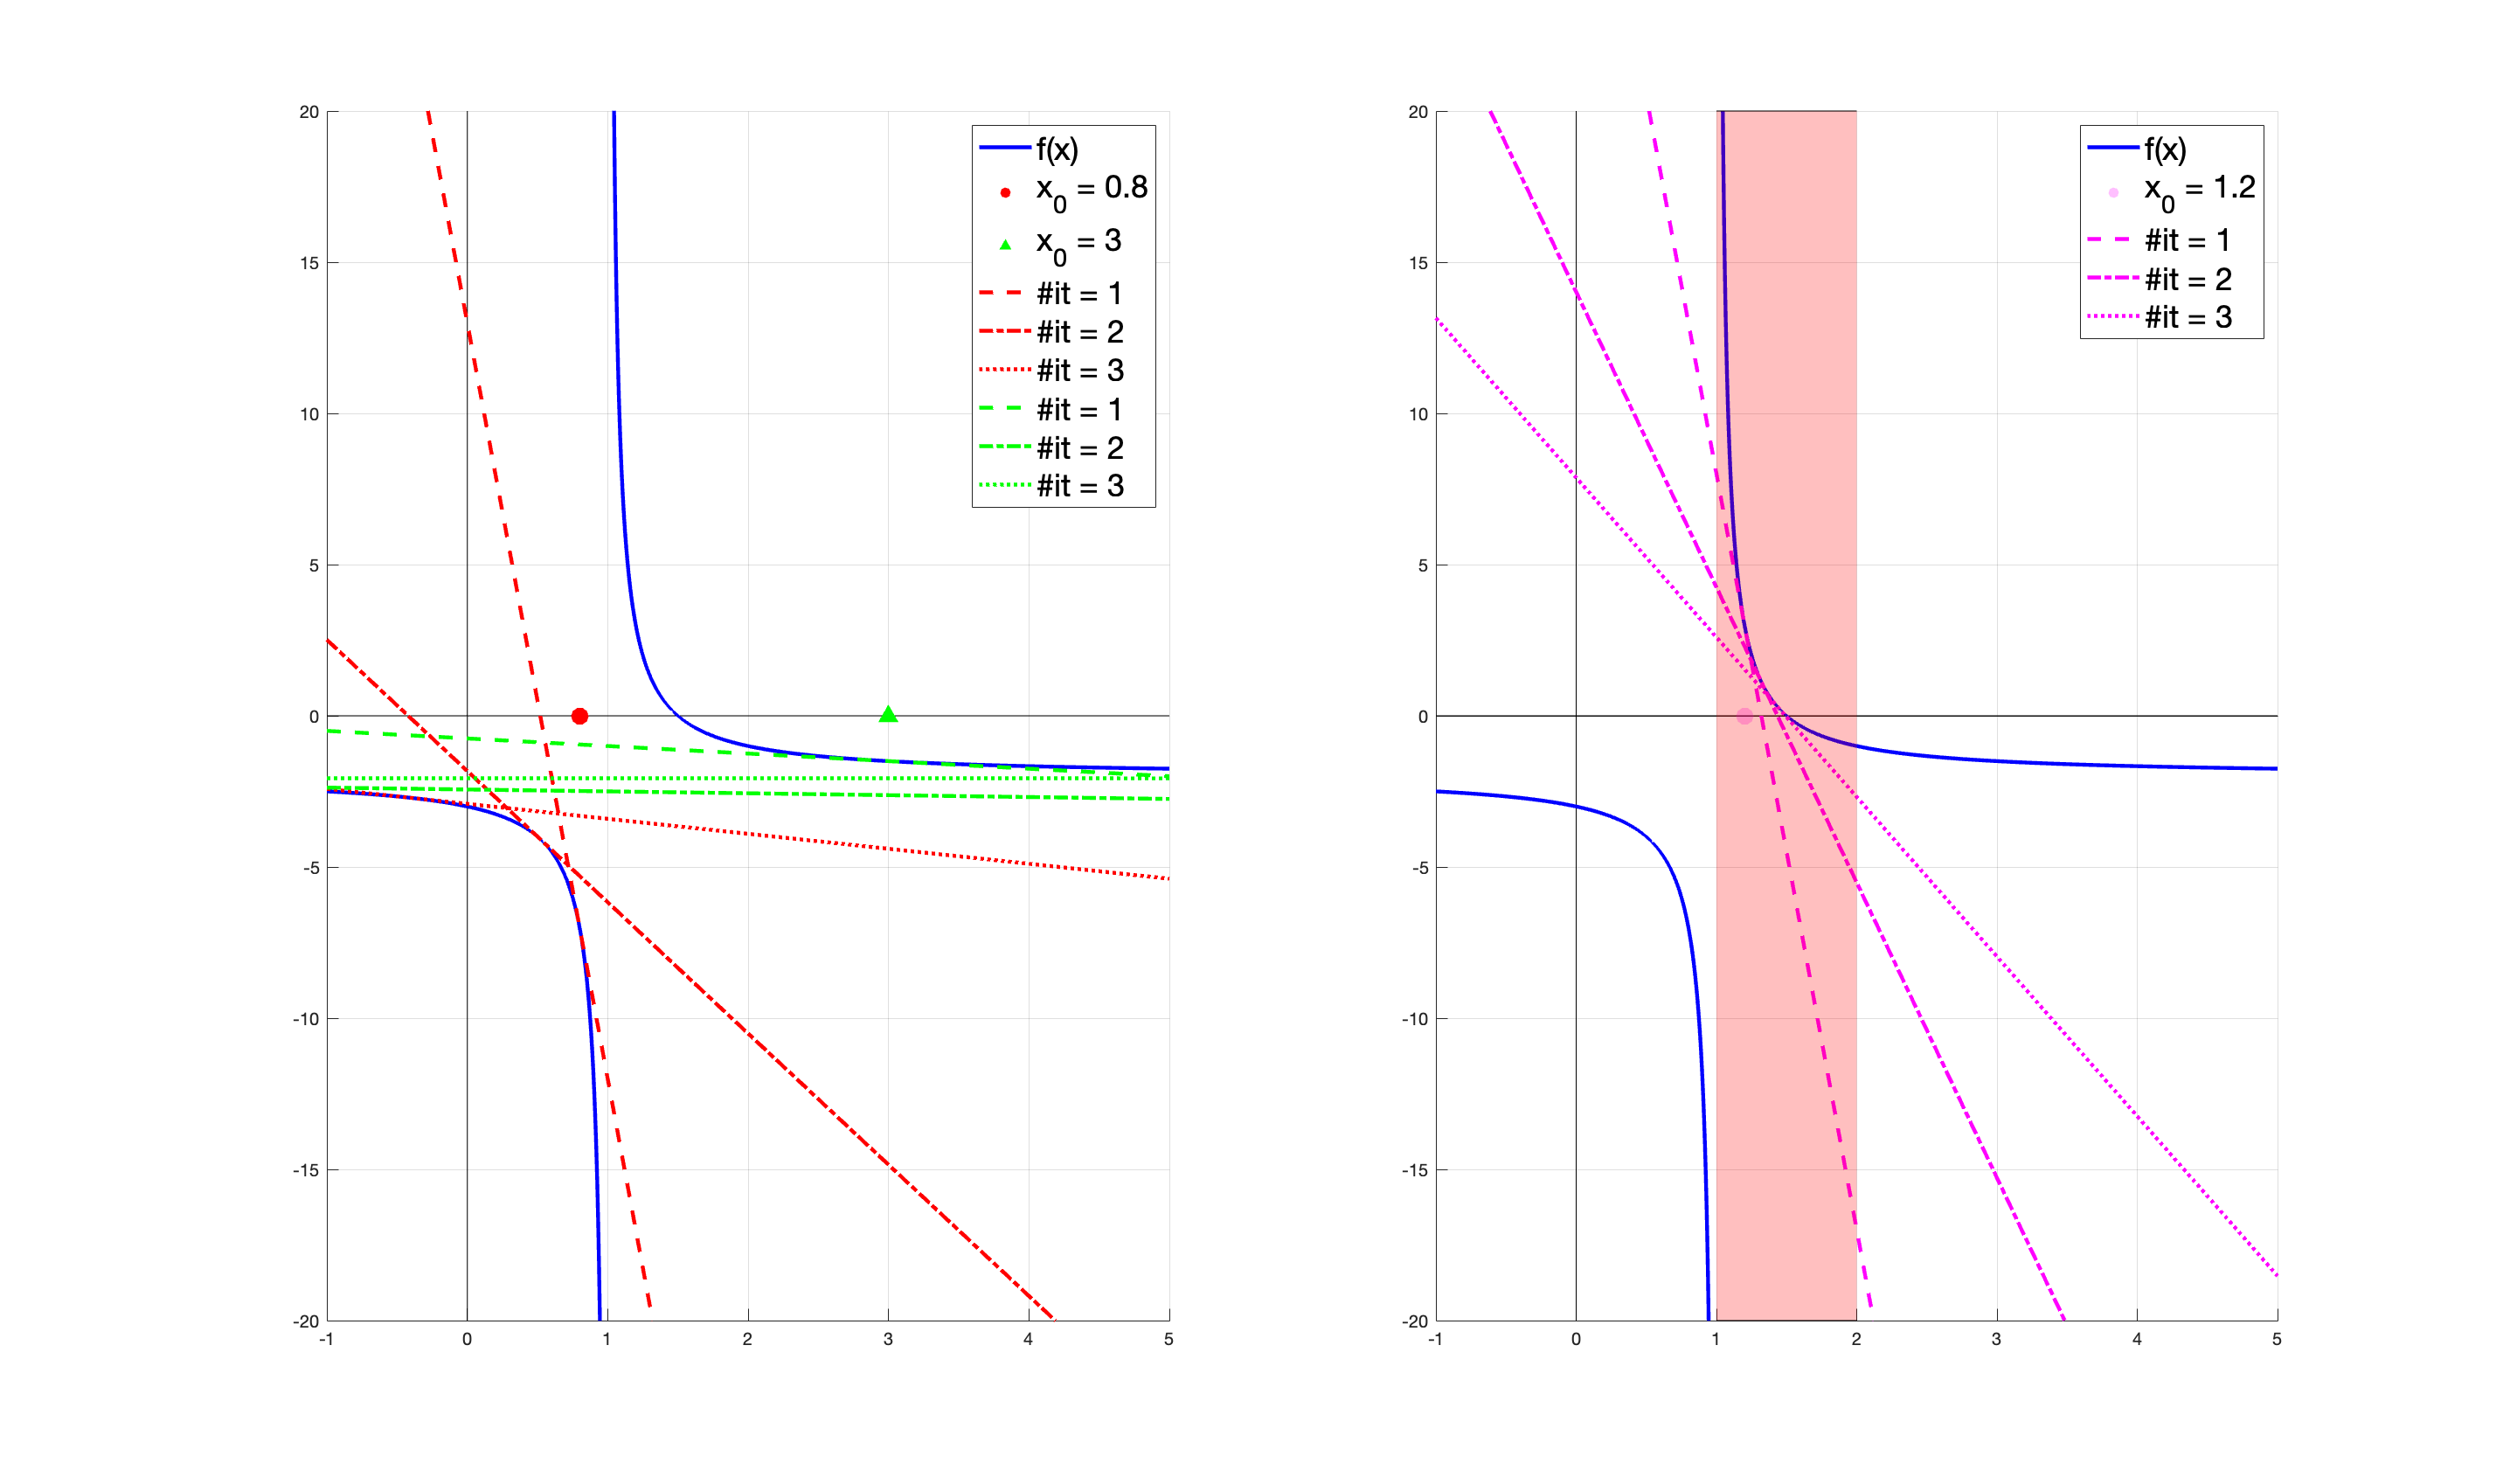
\includegraphics[width=1.\textwidth]{figures/newton_choose.png}
   \end{figure}
\end{frame}

\begin{frame}{}
   \begin{itemize}
      \item[$\blacktriangleright$] From the DIPPR\textsuperscript{\textregistered}
         database we learn that, for WATER ($H_{2}O$), the Vapor Pressure can be
         calculated In the range 273.16 K to 647.13 K as follows:
        \begin{equation*}
            P^{0}_{vap} (T) = exp\left(A + \frac{B}{T} + C \times ln(T) + D \times
            T^{E}\right ) \quad [Pa]
        \end{equation*}
         Where: $T$ is the temperature in Kelvin, $A = 7.3649e^{+01}$, $B =
         -7.2582e^{+03}$, $C = -7.3037e^{+00}$, $D = 4.1653e^{-06}$, $E = 2.0000e^{+00}$.
         Determine, using the newton method, for which temperature the vapor pressure is
         0.5 $atm$
   \end{itemize}
\end{frame}

\begin{frame}{}
   \begin{itemize}
      \item[$\blacktriangleright$] Write a function that calculates the bubble temperture
         of a binary blend of NC6 and NC7 (70/30 molar) at atmospheric pressure using a
         solver you developed (the solver will be a function that takes the function to
         be solved, the interval or the first guess needed to start the iterative
         procedure and the desired precision of the solution and returns the zero of the
         function. \textbf{Bubble Temperature of a mixture}.
         \begin{equation*}
            \sum_{i=1}^{NS} y_{i} = 1 \longrightarrow y_{i} = \frac{P_{i}^{0}(T)}{P}z_{i}
         \end{equation*}
         \begin{equation*}
            f(x) = 1 - \sum_{i=1}^{NS} \frac{P_{i}^{0}(T_{bubble})}{P}z_{i} = 0
         \end{equation*}
   \end{itemize}
\end{frame}

%%%%%%%%%%%%%%% CLOSING
{%
\setbeamertemplate{footline}{}
\begin{frame}[standout]
	Thank you for the attention!
\end{frame}
}

\end{document}
